\section{Recognition of Academic Software}
\label{study2}

The \textit{recognition of academic software} is concerned with the way of
academic software is visible by others scientists beyond its authors. 
A recognized academic software is the one mentioned by its peers in their papers,
that is, the one cited, evaluated (possibly against other software), used or
even modified by others.

\myparagraph{Scoping}
%
The goal of the study is to
analyze \textit{static analysis software projects published in the ASE and SCAM
papers} with the purpose of \textit{characterizing their recognizion}
concerning the \textit{number and types of mentions} in the perspective of
\textit{scientists} 
in the context of \textit{publications in the ACM and IEEE
digital libraries}. 

In this study, we investigated the following research question
regarding academic software for static analysis:

\newcommand{\StudyTwoQuestionOne} {
	\textbf{(RQ3.1)}\textit{How are the academic software projects for static analysis published
in ASE and SCAM papers \textit{mentioned} in ACM and IEEE publications?}
}

\noindent \StudyTwoQuestionOne We investigated how papers from the ACM
Digital Library and IEEE Xplore databases relate to the selected academic
software projects,  how many studies mention each project, and what is the type
of each found mention.

Measurements required in this study include 
the number of topical publications on ACM and IEEE that 
(1)~mention, (2)~use or (3)~contribute to, 
academic software for static analysis.
 
\myparagraph{Data Collection}
%
Our literature review found a total of \SearchUniqueCount \ papers 
on the ACM and IEEE digital libraries; 
among these publications, after inspection, 
we found \ScreeningUniqueCount \ papers\footnote{The list of all papers is available in the repository of this work at \url{https://github.com/joenio/dissertacao-ufba-2016/releases/download/2018-03-26/apendices.pdf}} \textit{mentioning} a subset of the \SoftwareCount \ academic software projects, as illustrated in Figure \ref{study2-literature-review}.
A {\it mention} means any occurrence of the name of the academic software
in a scientific publication, including even formal and informal citation.
We found these mentions in searches on the ACM and IEEE digital libraries 
carried out between July and August 2017.

\begin{figure}[ht]
  \center
  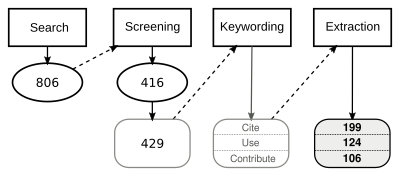
\includegraphics[scale=0.25]{figs/study2-literature-review.png}
  \caption{Number of publications and mentions at each step of literature review on ACM and IEEE bases.}
  \label{study2-literature-review}
\end{figure}

\myparagraph{Results and Analysis}
%
We have following implications:

\paragraph{\bf Mentions to academic software}
Regarding question \textbf{RQ3.1},
the \SoftwareCount \ academic software
projects for static analysis published by ASE and SCAM conferences are
mentioned \ScreeningCount \ times in \ScreeningUniqueCount \ distinct papers.
Only \SoftwareNotFoundOnSearch \ projects --
GUIZMO and protopurity -- were not found in
searches carried out in ACM and IEEE.
%
Among all mentions, three distinct types emerged concerning the level of
contribution to the ecosystem of the projects.
%
\textbf{(1) Citations:}
  describes the software;
  mentions the software in a table among others, classifies, cites as an example;
  and mentions as related work or future work.
%
\textbf{(2) Usages:}
  assesses or characterize the software;
  uses to collect and analysis of data; Uses as an object of study;
  uses the software as part of some proposed solution;
  and creates a new project based on the software without releasing it and contributions.
%
\textbf{(3) Contributions:}
  initial work publishing the software; Refactors the software;
  opens the source code of a software; Contributes to the source code; Extends the software;
  integrates the software to other systems, input/output file formats, APIs;
  and implements some features of the software on others projects and compares the results.
%
As detailed in Figure \ref{study2-literature-review}, most of them are ``citations''
 with \CiteCount \ mentions, followed by ``usages'' with \UseCount \ occurrences and ``contributions'' with \ContributeCount \ occurrences.

\paragraph{\bf Uses of academic software}
There are  \UseCount \ mentions that use an academic software 
as methodological support for collecting or analyzing data, 
as an object of study, or as a starting point to implement other research solutions.
%
We associated these ``usages'' mentions with 26 of the
\SoftwareCount \ software projects, 
indicating that less than half of academic
software projects for static analysis published in ASE and SCAM conferences 
are used by papers  retrieved from searches on ACM and IEEE databases.

\paragraph{\bf Contributions to academic software}
We found \ContributeCount \ mentions of type ``contributions''. 
This amount includes papers  that published academic software projects 
for the first time, i.e., software publications
that gave rise to the set of \SoftwareCount \ software
projects selected in our first exploratory study (Section~\ref{study1}).
%
When analyzing only contributions after the initial publication of the project,
that is, articles and studies contributing with source code to the projects
after their initial publication, we found \ContributeStudyDoisCount \ mentions
to a set of \ContributeStudyDoisSoftware \ software projects. 
That is, only 28\% of projects received source code contributions 
from studies after its initial publication, 
at least for studies from ACM and IEEE databases.

\myparagraph{Threats to validity}
%
We used a manual inspection to characterize the
mentions and their types, based on the reviewer's discretion. We used checklists
to help us in this inspection. The search conducted on two digital libraries
(ACM and IEEE)  may have left out work that mentions the investigated projects
since it is possible that there are publications not indexed by these bases.
